\documentclass[10pt,journal,compsoc]{IEEEtran}

\usepackage{cite}
\usepackage{amsmath,amssymb,amsfonts,amsthm,mathtools}
\usepackage{graphicx}
\usepackage{booktabs}
\usepackage{url}
\usepackage{tikz}
\usepackage{xr}
\externaldocument[supp-]{build/supplement}
\usetikzlibrary{arrows.meta,positioning,decorations.pathreplacing,automata,calc}
% Unified monochrome figure style for the paper.
% All automata and timing diagrams use white states, black borders and black arrows.
\tikzset{
  fmbracebottom/.style={
    decorate,
    decoration={brace,mirror,amplitude=4pt}
  },
  fmstate/.style={
    circle, draw=black, fill=white, line width=0.6pt,
    minimum size=9mm, inner sep=1pt, font=\small
  },
  fmstatewide/.style={
    rounded rectangle, draw=black, fill=white, line width=0.6pt,
    minimum height=8mm, inner xsep=3pt, inner ysep=1.5pt, font=\small
  },
  fmaccept/.style={fmstate,double,double distance=1.2pt},
  fmerror/.style={fmstate,double,double distance=1.2pt,fill=gray!12},
  fmedge/.style={->,>=Stealth,line width=0.6pt},
  fmlabel/.style={font=\scriptsize,align=center,fill=white,inner sep=1.2pt},
  fminvariant/.style={font=\scriptsize,align=center},
  fmnote/.style={font=\scriptsize,align=center},
  fmtimeline/.style={->,>=Stealth,line width=0.6pt},
  fmevent/.style={circle,draw=black,fill=white,line width=0.6pt,minimum size=4.5mm,inner sep=0.5pt},
  fmreference/.style={fmevent,double,double distance=0.8pt},
  fmguide/.style={densely dashed,line width=0.45pt},
  fmbrace/.style={decorate,decoration={brace,amplitude=4pt},line width=0.5pt}
}


\newtheorem{theorem}{Theorem}[section]
\newtheorem{lemma}[theorem]{Lemma}
\newtheorem{corollary}[theorem]{Corollary}
\newtheorem{proposition}[theorem]{Proposition}
\newtheorem{assumption}[theorem]{Assumption}
\newtheorem{definition}[theorem]{Definition}

\newcommand{\Nat}{\mathbb{N}}
\newcommand{\Real}{\mathbb{R}}
\newcommand{\satM}{\models_{\mathrm{MTL}}}
\newcommand{\satL}{\models_{\mathrm{LTL}}}
\newcommand{\Until}{\mathbin{\mathsf{U}}}
\newcommand{\Release}{\mathbin{\mathsf{R}}}
\newcommand{\hUntil}{\mathbin{\widehat{\mathsf{U}}}}
\newcommand{\hRelease}{\mathbin{\widehat{\mathsf{R}}}}
\newcommand{\Next}{\mathsf{X}}
\newcommand{\Always}{\mathsf{G}}
\newcommand{\Eventually}{\mathsf{F}}
\newcommand{\WeakUntil}{\mathbin{\mathsf{W}}}
\newcommand{\Reset}{\mathsf{rst}}
\newcommand{\Unch}{\mathsf{unch}}
\newcommand{\T}{\mathcal{T}}
\newcommand{\CVal}{\mathsf{val}}
\newcommand{\CReset}{\mathsf{reset}}
\newcommand{\elapsed}{\mathsf{elap}}
\newcommand{\Clock}{\mathit{Clock}}
\newcommand{\runinhead}[1]{\par\smallskip\noindent\textbf{#1}\enspace}

\title{A Mechanically Verified Translation of MTL$_{0,\infty}$ into Timed B\"uchi Automata}

\author{Elie Fares, Jean-Paul Bodeveix, Hussain Al-Aqrabi, and Azar Salami%
\thanks{Elie Fares, Hussain Al-Aqrabi, and Azar Salami are with the Higher Colleges of Technology, Sharjah, United Arab Emirates (e-mail: efares@hct.ac.ae; halaqrabi@hct.ac.ae; asalami@hct.ac.ae).}%
\thanks{Jean-Paul Bodeveix is with IRIT, Universit\'e de Toulouse, France (e-mail: bodeveix@irit.fr).}%
}

\begin{document}
\maketitle

\begin{abstract}
We present a Coq-verified translation from pointwise dense-time
$\mathrm{MTL}_{0,\infty}$ to timed B\"uchi automata. The translation first
reduces ordinary timed operators to strict hatted primitives, encodes their
timing constraints in clocked LTL, and then uses an arbitrary LTL-to-B\"uchi
backend satisfying an explicit semantic contract. A relaxation and reset
completion construction turns the backend automaton into a timed B\"uchi
automaton. The central proof difficulty is reuse: one clock is assigned to
each distinct primitive timed subformula, even when its obligation is
activated repeatedly and overlaps itself. We establish soundness and
completeness by a canonical reset policy and residual obligations, and prove
the end-to-end theorem \texttt{MTL\_to\_TBA\_correct\_with}. The result
preserves strict and non-strict bounds and does not depend on a particular
LTL-to-B\"uchi implementation.
\end{abstract}

\begin{IEEEkeywords}
Metric temporal logic, timed B\"uchi automata, Coq, formal verification,
clocked LTL, semantic preservation.
\end{IEEEkeywords}

\section{Introduction}
\label{sec:introduction}
Real-time requirements combine qualitative ordering with quantitative timing.
Metric Temporal Logic (MTL) expresses both, while timed B\"uchi automata (TBA)
provide a finite-state model suitable for timed verification. A translation
between them is useful only when the automaton preserves the pointwise
dense-time semantics of the formula. The translation itself is subtle: a
timed subformula nested under an unbounded temporal operator may be activated
without bound, and several instances of the same obligation may be pending at
once.

This paper gives a mechanized translation for the one-sided-bounded fragment
$\mathrm{MTL}_{0,\infty}$~\cite{[RK90],[RTH96],[BDLG14]}. Its key construction
assigns a clock to each \emph{distinct primitive timed subformula}, rather
than to each syntax-tree occurrence or run-time activation. The clocked-LTL
encoding constrains that shared clock through reset and preservation markers.
The proof's completeness direction chooses a canonical reset trace that
retains the oldest useful reference when it subsumes newer obligations;
residual predicates express what remains of an obligation after time has
advanced. This establishes that repeated activations need no additional
clocks.

The translation is factored through ordinary LTL. It is therefore independent
of the particular LTL-to-B\"uchi translator, subject only to a stated
correctness contract on propositional words. After the backend, relaxation
removes irrelevant negative extended-atom literals, and reset completion
turns the relaxed cubes into timed transitions. The resulting theorem is
mechanized in Coq for all eight hatted timed primitives, including strict
bounds. The proof does not cover parsing, the interface to an external LTL
translator, or output printing; these are outside the theorem.

Our contributions are:
\begin{itemize}
  \item a pointwise-semantics-preserving clocked-LTL encoding of the eight
        hatted Until and Release primitives, with ordinary timed operators
        derived by semantic identities;
  \item soundness and completeness of that encoding, including a canonical
        reset policy and residual obligations that justify one clock per
        distinct timed subformula despite arbitrarily overlapping activations;
  \item relaxation and reset completion, with an end-to-end Coq theorem for
        every LTL-to-B\"uchi backend satisfying the explicit correctness
        contract.
\end{itemize}

The formal development includes the named results
\texttt{EncodingCorrect\_proved}, \texttt{T\_uses\_every\_clock}, and
\texttt{MTL\_to\_TBA\_correct\_with}. The complete arguments for the
canonical policy and its strict-bound cases appear in the supplementary
material. This paper treats the translation through TBA construction; generic
TBA optimization and UPPAAL export are separate contributions and are not
needed for the theorem proved here.

\section{Logic and Semantic Model}
\label{sec:logic}
\subsection{Pointwise MTL$_{0,\infty}$}
\label{sec:mtl}
Let $\Sigma$ be a finite set of actions. Formulas are in negation normal
form and use Boolean operators, next, untimed Until and Release, and timed
Until and Release whose intervals have one endpoint at zero or infinity.
We write a bound as $\sim d$, with $\sim\in\{<,\le,>,\ge\}$. The logic also
contains the hatted operators $\hUntil_{\sim d}$ and
$\hRelease_{\sim d}$. In a hatted operator the current position is skipped
by the logical interval, while its timestamp remains the timing reference.

A timed word is $w=(a_i,t_i)_{i\in\Nat}$, where $a_i\in\Sigma$,
$0\le t_0<t_1<\cdots$, and timestamps diverge. We write
$\elapsed_w(i,j)=t_j-t_i$. For Until, $w,i\satM p\Until_{\sim d}q$
holds when some $j\ge i$ satisfies $q$ and $t_j-t_i\sim d$, with $p$ at
each position in $[i,j)$. For hatted Until, the witness is $j>i$ and $p$
is required on $(i,j)$. Release is the dual universal condition: at every
position in the bounded region, either $q$ holds or $p$ held earlier in the
corresponding interval. Hatted Release excludes the current position from
that region. We use the standard pointwise semantics~\cite{MTLsem}.

For precision, the four bounded clauses used below are:
\begin{align*}
 w,i\satM p\Until_{\sim d}q
 &\Longleftrightarrow \exists j\ge i.\; w,j\satM q\\
 &\quad\land t_j-t_i\sim d\\[-1mm]
 &\quad\land \forall k\in[i,j).\;w,k\satM p,\\
 w,i\satM p\hUntil_{\sim d}q
 &\Longleftrightarrow \exists j>i.\; w,j\satM q\\
 &\quad\land t_j-t_i\sim d\\[-1mm]
 &\quad\land \forall k\in(i,j).\;w,k\satM p,\\
 w,i\satM p\Release_{\sim d}q
 &\Longleftrightarrow \forall j\ge i.\\[-1mm]
 &\quad\Bigl(t_j-t_i\sim d\Rightarrow\\[-1mm]
 &\qquad\Bigl(w,j\satM q\\[-1mm]
 &\qquad\quad\lor \exists k\in[i,j).\;w,k\satM p\Bigr)\Bigr),\\
 w,i\satM p\hRelease_{\sim d}q
 &\Longleftrightarrow \forall j>i.\\[-1mm]
 &\quad\Bigl(t_j-t_i\sim d\Rightarrow\\[-1mm]
 &\qquad\Bigl(w,j\satM q\\[-1mm]
 &\qquad\quad\lor \exists k\in(i,j).\;w,k\satM p\Bigr)\Bigr).
\end{align*}
The index intervals refer to event positions, whereas $t_j-t_i$ is physical
time. This distinction is material when no event occurs exactly at a bound.
The strict increase assumption excludes simultaneous events; divergence is
used in the lower-bounded Until fairness argument.

The well-formedness condition requires $d>0$ for every lower bound and strict
upper bound, and $d\ge0$ for a non-strict upper bound. Ordinary timed
operators are definitions in the mechanized core. For upper bounds
$\precsim\in\{\le,<\}$ and lower bounds $\succsim\in\{\ge,>\},$ they are:
\begin{align}
p\Until_{\precsim d}q &\equiv q\lor(p\land(p\hUntil_{\precsim d}q)),\label{eq:derive-ule}\\
p\Until_{\succsim d}q &\equiv p\land(p\hUntil_{\succsim d}q),\label{eq:derive-uge}\\
p\Release_{\precsim d}q &\equiv q\land(p\lor(p\hRelease_{\precsim d}q)),\label{eq:derive-rle}\\
p\Release_{\succsim d}q &\equiv p\lor(p\hRelease_{\succsim d}q).\label{eq:derive-rge}
\end{align}
These definitions separate the current-position case from the strictly future
obligation. Their pointwise semantic compatibility, including the stated
bound hypotheses, is proved in Coq:
\begin{theorem}[Semantic compatibility of the derived timed operators]
\label{thm:derived-semantic-compatibility}
Under the well-formedness conditions above, Eqs.~\eqref{eq:derive-ule}--
\eqref{eq:derive-rge} agree with the standard pointwise semantics for all
strict and non-strict upper and lower bounds.
\end{theorem}
The identities follow by separating the current-position case from a
strictly future endpoint. For upper Until, a witness at $i$ contributes
$q$; every later witness requires $p$ at $i$ and leaves the hatted
obligation. A lower bound with $d>0$ excludes $i$, so $p$ is required now
and the remaining witness is hatted. The Release identities are the dual
case split: an upper-bound region includes $i$ and therefore requires $q$
there, while a lower-bound region excludes $i$. Strict upper bounds also
require $d>0$, avoiding the degenerate $<0$ case. The eight corresponding
Coq lemmas are listed in Supplement~\ref{supp-subsec:derived-operators-proof}.
Thus only
the eight hatted timed constructors require primitive translation clauses.

\begin{figure}[t]
\centering
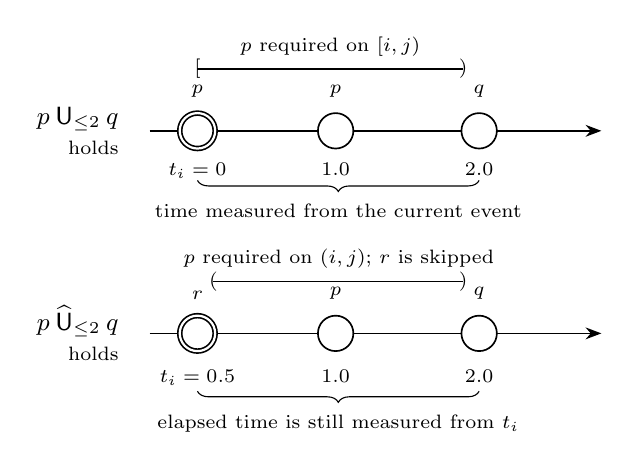
\begin{tikzpicture}[x=1.35cm,y=1.05cm,
  ival/.style={line width=0.5pt},
  ivallab/.style={font=\scriptsize,above=1pt}]
  % Ordinary Until
  \node[anchor=east,font=\small,align=right] at (-0.20,1.30) {$p\Until_{\le 2}q$\\{\scriptsize holds}};
  \draw[fmtimeline] (0,1.30) -- (4.25,1.30);
  \node[fmreference] (u0) at (0.45,1.30) {};
  \node[fmevent] (u1) at (1.75,1.30) {};
  \node[fmevent] (u2) at (3.10,1.30) {};
  \node[above=2pt of u0,font=\scriptsize] {$p$};
  \node[above=2pt of u1,font=\scriptsize] {$p$};
  \node[above=2pt of u2,font=\scriptsize] {$q$};
  \node[below=1.5pt of u0,font=\scriptsize] {$t_i=0$};
  \node[below=1.5pt of u1,font=\scriptsize] {$1.0$};
  \node[below=1.5pt of u2,font=\scriptsize] {$2.0$};
  \draw[ival] (0.45,2.05) -- (2.95,2.05);
  \node[font=\scriptsize] at (0.45,2.05) {$[$};
  \node[font=\scriptsize] at (2.95,2.05) {$)$};
  \node[ivallab] at (1.70,2.05) {$p$ required on $[i,j)$};
  \draw[fmbracebottom] (0.45,0.70) -- node[below=5pt,font=\scriptsize] {time measured from the current event} (3.10,0.70);

  % Hatted Until
  \node[anchor=east,font=\small,align=right] at (-0.20,-1.15) {$p\hUntil_{\le 2}q$\\{\scriptsize holds}};
  \draw[fmtimeline] (0,-1.15) -- (4.25,-1.15);
  \node[fmreference] (h0) at (0.45,-1.15) {};
  \node[fmevent] (h1) at (1.75,-1.15) {};
  \node[fmevent] (h2) at (3.10,-1.15) {};
  \node[above=2pt of h0,font=\scriptsize] {$r$};
  \node[above=2pt of h1,font=\scriptsize] {$p$};
  \node[above=2pt of h2,font=\scriptsize] {$q$};
  \node[below=3pt of h0,font=\scriptsize] {$t_i=0.5$};
  \node[below=3pt of h1,font=\scriptsize] {$1.0$};
  \node[below=3pt of h2,font=\scriptsize] {$2.0$};
  \draw[ival] (0.60,-0.52) -- (2.95,-0.52);
  \node[font=\scriptsize] at (0.60,-0.52) {$($};
  \node[font=\scriptsize] at (2.95,-0.52) {$)$};
  \node[ivallab] at (1.78,-0.52) {$p$ required on $(i,j)$; $r$ is skipped};
  \draw[fmbracebottom] (0.45,-1.85) -- node[below=5pt,font=\scriptsize] {elapsed time is still measured from $t_i$} (3.10,-1.85);
\end{tikzpicture}

\caption{Ordinary and hatted Until. The double circle is the timing reference.
The hatted operator skips the current event logically but measures from its
timestamp.}
\label{fig:hatted-until}
\end{figure}

This distinction is useful for sporadicity: if consecutive occurrences of
$e$ must be separated by at least $\theta$, one may write
$\Box(e\Rightarrow\widehat{\Box}_{<\theta}\neg e)$. The hatted form retains
the triggering event as the time origin; ordinary bounded temporal
operators do not express this particular reference shift directly.
Related pointwise MTL constructions and the CASAAL translation are discussed
in prior work~\cite{ouaknine_worrell_lics05,bouyer_chevalier_markey_fsttcs05,li_spin7,casaal_tool}.

\subsection{Timed B\"uchi Automata}
\label{sec:tba}
A TBA is a tuple $\mathcal A=(L,\ell_0,X,E,\mathit{Acc},\mathit{Inv})$.
Here $L$ is a finite set of locations, $X$ a finite set of clocks,
$E\subseteq L\times\mathsf{Lab}\times\mathsf{Guard}\times 2^X\times L$
is a set of action-labelled transitions with guards and reset sets,
$\mathit{Acc}\subseteq L$ is the B\"uchi set, and $\mathit{Inv}$ assigns a
clock constraint to each location. A run on a timed word follows one
transition per event, respects the invariant throughout each delay, tests
guards at the event, and resets exactly the clocks on the transition.
Acceptance requires infinitely many visits to $\mathit{Acc}$. For the
translation theorem below, the initial clock values are existentially
quantified. This matches the clock-consistent-extension semantics used by
the Coq development; conventional zero initialization is a separate
property. More explicitly, let $v_i$ be the valuation tested at event $i$,
and let $\Delta_i=t_{i+1}-t_i$. A run is an infinite sequence
$(\ell_i,v_i)_{i\ge0}$ with an initial nonnegative valuation $v_0$. At
event $i$, it chooses $(\ell_i,\alpha,g,Z,\ell_{i+1})\in E$ such that the
action satisfies $\alpha$, the event valuation satisfies $g$, and the
invariant of $\ell_i$ holds throughout the delay since the preceding event.
The post-transition valuation is
\[
v_{i+1}(x)=
\begin{cases}
\Delta_i,&x\in Z,\\
v_i(x)+\Delta_i,&x\notin Z,
\end{cases}
\]
and must satisfy $\mathit{Inv}(\ell_{i+1})$. For $i>0$, the delay is
$t_i-t_{i-1}$; the first event's pre-event valuation is existential. This
event-indexed convention makes TBA clock values correspond directly to the
clock values of an extended word.

\section{Clocked-LTL Translation}
\label{sec:translation}
\subsection{Shared clock identities}
The translation is structural. It maps Boolean and untimed temporal
operators homomorphically and maps each primitive timed subformula to an LTL
formula over an extended alphabet. The extended alphabet contains action
atoms, clock comparisons $x\sim d$, a reset atom $\Reset(x)$, and a
preservation atom $\Unch(x)$. These last atoms describe the clock update at
the current event. Clock values are read before the event's reset, matching
the guard semantics of a timed automaton.

For formula $f$, let $\Clock(f)$ be its finite set of distinct primitive
hatted timed subformulas. The clock associated with $F\in\Clock(f)$ is
$x=F$ itself. Thus two identical timed subformulas at different syntax-tree
paths denote the same logical clock. Syntactically different subformulas
remain distinct in this construction. The main result proves that the clock
also serves all dynamic activations of that subformula.
The clock count is therefore bounded by the number of distinct primitive
timed subformulas, which is at most the number of timed occurrences in $f$.
If structural subformulas are represented as shared nodes, the translation
can share their LTL encodings as well; this does not remove the usual
worst-case growth of an LTL-to-B\"uchi construction.

This sharing is semantic rather than an automaton-state minimization. The
clock key is the normalized primitive formula, including its comparison and
constant, so identical obligations have one clock identity before the
propositional automaton is built. The reset trace is then chosen for that
identity as a whole. In particular, the proof cannot justify the clock bound
by assigning a fresh clock to each activation and subsequently identifying
those clocks: it establishes directly that a single trace of reset decisions
for the formula is sufficient.

\subsection{Eight primitive clauses}
\label{sec:mtlbuchi}
Let $F$ be a primitive hatted formula at path $\pi$, with operands $p,q$.
Write $x=\mathsf{clock\_of}(F)$, $P=\T_{\pi0}(p)$,
$Q=\T_{\pi1}(q)$, and define
$\alpha\WeakUntil\beta=(\alpha\Until\beta)\lor\Always\alpha$.
For upper comparisons $\precsim\in\{\le,<\}$ and lower comparisons
$\succsim\in\{\ge,>\}$, complements are
$\le^{\mathrm c}=>$, $<^{\mathrm c}=\ge$, $\ge^{\mathrm c}=<$, and
$>^{\mathrm c}=\le$. The four clause shapes, each instantiated for its
strict and non-strict bound, give all eight primitive cases:
\begin{align}
\T_\pi(p\hUntil_{\precsim d}q)
 &=\Next\bigl(((x\precsim d)\land\Unch(x)\land P)\nonumber\\
 &\hspace{23mm}\WeakUntil((x\precsim d)\land Q)\bigr),\label{eq:t-hule}\\
\T_\pi(p\hUntil_{\succsim d}q)
 &=\Reset(x)\land\Next\bigl((P\Until((x\succsim d)\land(P\Until Q)))\nonumber\\
 &\hspace{23mm}\lor(\Always P\land\Always\Eventually Q)\bigr),\label{eq:t-huge}\\
\T_\pi(p\hRelease_{\precsim d}q)
 &=\Reset(x)\land\Next\bigl(Q\nonumber\\
 &\hspace{23mm}\WeakUntil((x\mathrel{\precsim^{\mathrm c}}d)\lor(P\land Q))\bigr),\label{eq:t-hrle}\\
\T_\pi(p\hRelease_{\succsim d}q)
 &=\Next\bigl(((x\mathrel{\succsim^{\mathrm c}}d)\land\Unch(x))\nonumber\\
 &\hspace{23mm}\WeakUntil((P\Release Q)\lor((x\mathrel{\succsim^{\mathrm c}}d)\land P))\bigr).
 \label{eq:t-hrge}
\end{align}
All clock atoms occur positively. Upper-bounded hatted Until uses weak
Until because a clock-consistent trace must eventually cross its finite
upper bound if no endpoint is found. Lower-bounded Until retains its
fairness branch, including $\Always\Eventually Q$, so that eventuality is
not lost. The other weak-Until clause marks the end of a bounded Release
window. Strict comparisons are represented directly; no strict bound is
weakened by adjusting its constant.

The clauses have four distinct temporal roles. For upper-bounded Until, the
clock is tested before any new reset: while its value remains in the allowed
window, $P$ must continue until $Q$ appears; if the bound is passed first,
the weak-until tail requires the continuation to remain valid. For
lower-bounded Until, a finite path waits for the threshold and then starts
the unbounded $P\Until Q$ obligation. If the threshold is never reached,
the second disjunct requires $P$ at every position and $Q$ infinitely often.
Time divergence is what makes this infinite branch equivalent to a witness
at distance at least $d$.

For upper-bounded Release, the initial $Q$ is required and the weak-until
stops either at the complementary clock comparison or when $P\land Q$
discharges the obligation. For lower-bounded Release, the clock remains
unchanged before the threshold; after that point, the translated obligation
is ordinary Release, with the endpoint alternative covering the transition
into the threshold region. Thus Until clauses use existential witnesses,
whereas Release clauses maintain a universal condition over the bounded
region. The hatted shift is encoded by the outer $\Next$ in every clause;
for restart families, the separate $\Reset(x)$ atom denotes the reference
timestamp at the current position.

\begin{table}[t]
\centering
\caption{Clock comparisons used by each hatted primitive.}
\label{tab:clock-tests}
\footnotesize
\begin{tabular}{@{}lll@{}}
\toprule
Primitive role & Non-strict bound & Strict bound\\
\midrule
$\hUntil_{\precsim d}$ endpoint & $x\le d$ & $x<d$\\
$\hUntil_{\succsim d}$ threshold & $x\ge d$ & $x>d$\\
$\hRelease_{\precsim d}$ window end & $x>d$ & $x\ge d$\\
$\hRelease_{\succsim d}$ pre-threshold & $x<d$ & $x\le d$\\
\bottomrule
\end{tabular}
\end{table}

\subsection{Why hatted operators and shared clocks matter}
The hatted operators preserve the triggering timestamp while moving logical
evaluation to the next event. The same distinction appears in the clocked
encoding: the initial $\Next$ moves the temporal obligation forward, while
the clock retains the reference selected by its reset trace.

Clock sharing has two layers. First, identical primitive formulas at
different syntax-tree paths share one clock by construction. Second, that
single clock must represent all pending activations. For example, in
$\Box(\mathit{req}\Rightarrow\Diamond_{\le5}\mathit{ack})$, requests at times
0 and 2 can both be pending before an acknowledgement. Retaining the
reference from time 0 suffices: an acknowledgement at time 4 is within five
time units of both requests. Table~\ref{tab:overlap-example} traces this
case. Clock values are measured before the reset decision at each event; at
the acknowledgement, the guard sees age four and the successful endpoint
discharges both activations. For any newer request at time $t_k$ between an
older activation $t_i$ and a witness $t_j$, $t_j-t_k\le t_j-t_i$; the same
endpoint therefore satisfies the newer upper-bound obligation. The argument
depends on the required $P$ condition holding between activations and the
endpoint, which is exactly what the Until residual records.

\begin{table}[t]
\centering
\caption{One shared upper-Until clock for overlapping requests.}
\label{tab:overlap-example}
\footnotesize
\begin{tabular}{@{}clcc@{}}
\toprule
Event $i$ & Action & Time $t_i$ & Clock age before decision\\
\midrule
0 & $\mathit{req}$ & 0 & 0\\
1 & $\mathit{req}$ & 2 & 2\\
2 & $\mathit{ack}$ & 4 & 4\\
\bottomrule
\end{tabular}
\end{table}

For the other primitive families, the canonical policy and residual
predicates handle the direction in which restarting or preserving the clock
is required (Supplement~\ref{supp-subsec:residuals}).

\subsection{Canonical reset policy}
\label{subsec:canonical-main}
The encoding quantifies over clock traces. To prove completeness with one
clock for a formula that may be activated arbitrarily often, it is enough to
construct one trace that gives priority to an older activation only while
that activation remains useful. The proof records usefulness by residual
obligations. For upper-bounded Until, the residual says that a witness is
still reachable from the current clock age:
\begin{align*}
\mathsf{URes}_{\precsim}(i,v,d,p,q)\iff
\exists j\ge i.\;&v+\elapsed_w(i,j)\precsim d\\[-1mm]
&\land\ w,j\satM q\\[-1mm]
&\land\ \forall k\in[i,j).\\[-1mm]
&\qquad w,k\satM p,
\end{align*}
where $\precsim$ is either $\le$ or $<$. For lower-bounded Release, the
residual records that every position beyond the threshold is still covered:
\begin{align*}
\mathsf{RRes}_{\ge}(i,v,d,p,q)\iff
\forall j\ge i.\;&d\le v+\elapsed_w(i,j)\Rightarrow\\[-1mm]
&\Bigl(w,j\satM q\\[-1mm]
&\qquad\lor\exists k\in[i,j).\\[-1mm]
&\qquad\qquad w,k\satM p\Bigr),\\
\mathsf{RRes}_{>}(i,v,d,p,q)\iff
\forall j\ge i.\;&d<v+\elapsed_w(i,j)\Rightarrow\\[-1mm]
&\Bigl(w,j\satM q\\[-1mm]
&\qquad\lor\exists k\in[i,j).\\[-1mm]
&\qquad\qquad w,k\satM p\Bigr).
\end{align*}
The strict predicates preserve the strict comparison itself. They are
defined and shifted in the Coq development (the full definitions and
one-step lemmas are in Supplement~\ref{supp-subsec:residuals}).

The residual predicates are deliberately asymmetric. An upper-Until residual
is existential: one still-reachable endpoint is enough, and that endpoint
can discharge the obligation initiated at the current position. A
lower-Release residual is universal: every position that has entered the
threshold region must satisfy the Release condition. The canonical policy
preserves a clock only when its residual remains true, so clock reuse follows
from the semantic shape of the obligation rather than a syntactic rule such
as “reset on every activation.” This distinction is needed for repeated
activations, but the policy is not part of the generated automaton: it is a
word-dependent witness used only to prove completeness.

For clock $x=F$ with current value $v$, the canonical policy is summarized
in Table~\ref{tab:canonical-policy}. ``Preserve iff'' means that the clock is
not reset exactly under the listed condition; in the remaining cases it is
reset. For the restart families, the stated test is the reset condition.
\begin{table}[t]
\centering
\caption{Canonical reset policy for each timed-operator family.}
\label{tab:canonical-policy}
\footnotesize
\begin{tabular}{@{}p{0.34\columnwidth}p{0.60\columnwidth}@{}}
\toprule
Primitive clock $F$ & Reset decision at position $i$\\
\midrule
$p\hUntil_{\le d}q$ &
Preserve iff $v\le d$, $\mathsf{URes}_{\le}(i,v,d,p,q)$, and
$w,i\not\satM q$.\\
$p\hUntil_{<d}q$ &
Preserve iff $v<d$, $\mathsf{URes}_{<}(i,v,d,p,q)$, and
$w,i\not\satM q$.\\
$p\hUntil_{\ge d}q$, $p\hUntil_{>d}q$,
$p\hRelease_{\le d}q$, $p\hRelease_{<d}q$ &
Reset iff $w,i\satM F$.\\
$p\hRelease_{\ge d}q$ &
Preserve iff $v<d$, $\mathsf{RRes}_{\ge}(i,v,d,p,q)$, and
$w,i\not\satM p$.\\
$p\hRelease_{>d}q$ &
Preserve iff $v\le d$, $\mathsf{RRes}_{>}(i,v,d,p,q)$, and
$w,i\not\satM p$.\\
\bottomrule
\end{tabular}
\end{table}
The canonical extension uses this decision for the formula-keyed clock and
updates its value by
\[
u_0=0,\qquad
u_{i+1}=
\begin{cases}
\Delta_i,&\text{if the policy resets at }i,\\
u_i+\Delta_i,&\text{otherwise.}
\end{cases}
\]
The policy depends on truth in the timed word and, through residuals, on its
future. It is a semantic witness used in the completeness proof, not an
algorithm executed by the translator. Its input is the timed formula itself,
not a syntax-tree path, so identical occurrences share the same reset trace.

The two preservation cases retain an older reference only if the residual
is still true and the current event has not discharged it. A later endpoint
that satisfies the older upper-bounded Until also satisfies newer pending
copies with shorter remaining prefixes. For lower-bounded Release, an old
reference reaches the threshold no later than a newer one; the residual
shift $(i,v)\mapsto(i+1,v+\Delta_i)$ carries the remaining obligation.
Conversely, lower-bounded Until and upper-bounded Release restart when the
current formula is true; their translated continuation keeps any older
obligations represented. The strict cases follow the same organization with
strict residuals and guards.

\section{From Clocked LTL to a TBA}
\label{sec:tba-construction}
\subsection{LTL-to-B\"uchi contract}
The backend treats extended atoms as independent propositions. It returns a
propositional B\"uchi automaton whose language is exactly that of the
clocked-LTL formula. The theorem is stated for any such backend, deterministic
or not.
\begin{assumption}[Backend correctness]
\label{ass:backend}
For each formula $F$ and each propositional word $s$ over its atoms,
$\mathsf{PBA\_accepts}(A,s)$ iff $s,0\models F$, where $A$ is the backend
automaton for $F$.
\end{assumption}
This contract ranges over all propositional words, including assignments
that do not correspond to any clock-consistent timed word. That stronger
scope is used by relaxation.

\subsection{Relaxation and reset completion}
\label{sec:reset-completion}
The clocked-LTL formula has positive occurrences of extended atoms. Its
propositional language is consequently upward closed in those atoms. In each
backend cube, relaxation deletes negative literals over extended atoms and
irrelevant extended atoms; contradictory cubes are discarded. This preserves
the accepted language because any satisfying assignment can be adjusted to
the original cube while remaining a model of the positive formula.

Each clock belongs to one of two classes. A preservation clock is used with
upper-bound tests and $\Unch(x)$, and a restart clock is used with
lower-bound tests and $\Reset(x)$. Reset completion converts a relaxed cube
into a TBA transition as follows:
\begin{itemize}
  \item reset a preservation clock unless the cube contains $\Unch(x)$;
  \item reset a restart clock exactly when the cube contains $\Reset(x)$;
  \item remove reset and preservation markers, retaining clock tests as the
        transition guard and action literals as its label.
\end{itemize}
The asymmetry is essential. Additional resets only decrease preservation
clock values and hence preserve upper tests. A restart clock can be reset
only when explicitly required, since decreasing it could invalidate a lower
test. The full monotonicity argument is given in
Supplement~\ref{supp-subsec:reset-completion-proof}.

\begin{lemma}[Reset completion]
\label{lem:reset-completion}
For every accepting run of the relaxed backend automaton on a
clock-consistent extension, there is a clock-consistent extension with the
same timed word and initial values whose resets are exactly those prescribed
by reset completion, and the same run is accepting in the resulting TBA.
\end{lemma}

\begin{proposition}[Exactness of relaxation and reset completion]
\label{prop:reset-completion}
Let $f$ be well formed and let $A$ satisfy Assumption~\ref{ass:backend}
for $\T(f)$. The TBA obtained from $A$ by relaxation and reset completion
accepts exactly the timed words $w$ for which $w,0\satM f$, under
existential initial clock values.
\end{proposition}
The relaxation proof uses positivity of the clock atoms in $\T(f)$. A run
of the original B\"uchi automaton remains a run after relaxation. In the
reverse direction, take a run of the relaxed automaton and adjust each
propositional assignment only on the extended atoms whose negative literals
were deleted, making those atoms false; set irrelevant deleted atoms to true
where needed to recover the original cube. The backend contract makes the
adjusted word a model of $\T(f)$. On atoms that occur in $\T(f)$, the
relaxed word only adds truth, so upward closure makes it a model too.
Reset completion then assigns resets monotonically: preservation clocks
become no larger, keeping upper guards true, and restart clocks become no
smaller, keeping lower guards true. Thus the same B\"uchi run remains
accepting. The proof is mechanized as
\texttt{relax\_sound}, \texttt{relax\_complete}, and
\texttt{complete\_complete}.

\runinhead{Acceptance convention.}
The theorem quantifies existentially over the nonnegative clock values at
the first event. This is a property of the accepted timed language; it does
not by itself establish equivalence with an automaton whose clocks must
start at zero. For example, a first transition guarded by $x\ge1$ may be
enabled for one existential initial value and disabled when the first event
is at time zero. The conventional initialization question is therefore
outside Theorem~\ref{thm:mtl-to-tba-correct}; the Coq result is stated for
the existential convention used throughout the translation proof.

\section{Correctness and Clock Bound}
\label{sec:correctness}
\label{sec:encoding-correctness}
An extended word $\rho$ adds, at every position $i$, a value
$\CVal_\rho(i,x)\in\Real_{\ge0}$ and reset decision
$\CReset_\rho(i,x)$ for each $x\in\Clock(f)$. It is clock-consistent when,
for $\Delta_i=t_{i+1}-t_i$,
\begin{equation}
\CVal_\rho(i+1,x)=
\begin{cases}
\Delta_i,&\CReset_\rho(i,x),\\
\CVal_\rho(i,x)+\Delta_i,&\text{otherwise.}
\end{cases}
\label{eq:clock-update}
\end{equation}
The value at position $i$ is the value tested by guards before the reset
decision at that position. Let $\mathsf{same\_base}(\rho,w)$ mean that $w$
is the timed-word projection of $\rho$.

\begin{theorem}[Correctness of the clock encoding]
\label{thm:encoding-correctness}
For every well-formed formula $f$ and timed word $w$,
\begin{align*}
w,0\satM f\quad\Longleftrightarrow\quad
\exists\rho.\;&\mathsf{same\_base}(\rho,w)\\[-1mm]
&\land\ \mathsf{clock\_consistent}(\rho)\\[-1mm]
&\land\ \rho,0\satL\T(f).
\end{align*}
\end{theorem}
The existential quantifier over $\rho$ is taken jointly over all distinct
timed subformulas. Soundness does not rely on choosing the canonical trace:
each clock may follow any reset pattern allowed by the encoding, provided its
value recurrence is respected. Completeness is the more delicate half
because all activations that share a formula-keyed clock must be served
simultaneously. The proof constructs the clock traces in parallel, using the
residual predicates only for the preservation families and the direct
restart rule for the remaining families.
This result is the Coq theorem \texttt{EncodingCorrect\_proved}. Its
soundness direction holds for any clock-consistent reset trace. Completeness
constructs one canonical trace for all clocks together. The detailed
induction, including the strict-bound arithmetic, is in
Supplement~\ref{supp-sec:supp-proof}.

\begin{corollary}[One clock per distinct primitive timed subformula]
\label{cor:one-clock-formula}
All occurrences of the same primitive timed subformula use the same logical
clock. The encoding uses exactly the clocks in $\Clock(f)$, hence at most
one clock per distinct primitive timed subformula, independently of the
number of syntax-tree occurrences or run-time activations.
\end{corollary}
\begin{proof}
Every clock in $\T(f)$ is indexed by an element of $\Clock(f)$, and
\texttt{T\_uses\_every\_clock} proves that every such element occurs in
$\T(f)$. A single extension assigns one value and reset trace to each
element of $\Clock(f)$. Theorem~\ref{thm:encoding-correctness} proves that
the canonical trace suffices for every pending activation of that formula.
\end{proof}

Define $\mathsf{compile\_with}(A)$ by applying relaxation and reset
completion to backend automaton $A$. Timed acceptance is existential over
clock-consistent extensions of the timed word and requires that reset
decisions agree with the reset sets along an accepting run.
\begin{theorem}[MTL-to-TBA correctness]
\label{thm:mtl-to-tba-correct}
\label{cor:mtl-tba-correct}
For every well-formed $f$, backend automaton $A$ satisfying
Assumption~\ref{ass:backend}, and timed word $w$,
\[
w,0\satM f\quad\Longleftrightarrow\quad
\mathsf{TBA\_accepts}(\mathsf{compile\_with}(A),w).
\]
In Coq this is \texttt{MTL\_to\_TBA\_correct\_with}; the backend
correctness is an explicit hypothesis, not a project-specific axiom.
\end{theorem}
\begin{proof}
Combine Theorem~\ref{thm:encoding-correctness} with
Proposition~\ref{prop:reset-completion}. The forward direction uses the
canonical extension and reset-completion lemma; the reverse direction uses
upward closure under relaxation, the backend contract, and clock-encoding
soundness.
\end{proof}

\subsection{Proof structure}
\label{subsec:proof-outline}
The Coq proof separates the translation into local timed reasoning and
structural composition. The local lemmas cover only the eight hatted
constructors; Boolean, next, untimed Until and Release follow by induction.
The ordinary timed operators have already been unfolded by the semantic
identities, so they introduce no additional clock case. The full case-by-case
proof and arithmetic lemmas are in Supplement~\ref{supp-sec:supp-proof}.

\runinhead{Policy-independent soundness.}
Clock consistency supplies two inequalities. If $x$ is not reset on
$[i,j)$, then
$\CVal_\rho(j,x)=\CVal_\rho(i,x)+\elapsed_w(i,j)$, so its age at $j$ is at
least the physical time elapsed since $i$. If $x$ was reset at $i$, then
$\CVal_\rho(j,x)\le\elapsed_w(i,j)$; any subsequent reset only decreases
its age. Thus an upper guard at a preserved endpoint entails the matching
upper bound on elapsed time, while a lower guard after a reset entails the
matching lower bound. The inequalities preserve strictness: $x<d$ implies
elapsed time $<d$, and $x>d$ implies elapsed time $>d$.

For upper-bounded hatted Until, the LTL Until provides an endpoint, its
clock guard bounds the distance, and the translated left operand supplies
the open-interval prefix. Lower-bounded hatted Until has a finite branch
with a threshold guard and an infinite branch
$\Always P\land\Always\Eventually Q$. The finite branch gives the lower
bound directly; in the infinite branch, divergence supplies a sufficiently
late $q$ witness. For strict lower bounds, strict monotonicity between
positions $i$ and $i+1$ upgrades the distance from the $i+1$ tail to a
strictly greater distance from the original reference. The two Release
families use weak Until to express a bounded window: upper-bounded Release
ends when the complementary upper test becomes true or when $p\land q$
discharges the obligation; lower-bounded Release preserves its clock before
the threshold until either $p$ discharges it or ordinary Release takes over.
These arguments use no property of the reset policy beyond clock
consistency.

\runinhead{Completeness with one trace per formula.}
Completeness uses the canonical extension from
Definition~\ref{supp-def:canonical-policy}; the extension is shared by all
occurrences and activations of each formula-keyed clock. For upper-bounded
Until, the induction maintains, up to a selected endpoint $j$,
\[
\CVal_{\rho^\star}(n,x)+\elapsed_w(n,j)\precsim d.
\]
If an older reference remains useful, its residual ensures this inequality
continues to hold and also covers newer activations. Otherwise the policy
resets and starts the current obligation with the required remaining
budget. The first suitable $q$ endpoint closes the weak-until requirement.
The strict case uses the strict invariant with $<d$.

For lower-bounded Until, each activation of a true formula resets its clock.
If a threshold is reached, the finite branch of the translated formula
continues with $P\Until Q$. If it is never reached, the active-obligation
invariant implies that $p$ persists and $q$ recurs, yielding the fairness
branch. For upper-bounded Release, restarting at a true activation lets the
weak-until clause track the current bounded window until $p\land q$ or the
complementary clock test ends it. For lower-bounded Release, the invariant
is the corresponding residual predicate; while the policy preserves the
clock, its value advances by $\Delta_i$, and the residual shifts from
$(i,v)$ to $(i+1,v+\Delta_i)$. That shift retains the coverage of every
position beyond the threshold. These cases establish the translated
formula at each syntactic occurrence by induction, while the clock key
identifies duplicate timed subformulas.

\begin{table}[t]
\centering
\caption{Coq lemmas for the primitive timed proof cases. Each row denotes
both strict and non-strict comparisons.}
\label{tab:primitive-proof-lemmas}
\footnotesize
\begin{tabular}{@{}lll@{}}
\toprule
Primitive family & Soundness & Canonical completeness\\
\midrule
$\hUntil_{\le d}$ & \texttt{sound\_UhatLe} & \texttt{complete\_UhatLe}\\
$\hUntil_{\ge d}$ & \texttt{sound\_UhatGe} & \texttt{complete\_UhatGe}\\
$\hRelease_{\le d}$ & \texttt{sound\_RhatLe} & \texttt{complete\_RhatLe}\\
$\hRelease_{\ge d}$ & \texttt{sound\_RhatGe} & \texttt{complete\_RhatGe}\\
$\hUntil_{<d}$ & \texttt{sound\_UhatLt} & \texttt{complete\_UhatLt}\\
$\hUntil_{>d}$ & \texttt{sound\_UhatGt} & \texttt{complete\_UhatGt}\\
$\hRelease_{<d}$ & \texttt{sound\_RhatLt} & \texttt{complete\_RhatLt}\\
$\hRelease_{>d}$ & \texttt{sound\_RhatGt} & \texttt{complete\_RhatGt}\\
\bottomrule
\end{tabular}
\end{table}

The local cases are assembled into the theorem
\texttt{EncodingCorrect\_proved}. Its completeness argument proves
equivalence for every node identified by a syntax-tree path, not only for
the root. This stronger induction invariant is needed because repeated
formula occurrences share the same clock while the induction traverses
separate paths.

\runinhead{What the mechanization assumes.}
The proof boundary is summarized in Table~\ref{tab:proof-boundary}. In
particular, the correctness of the untimed backend is an explicit
proposition-level assumption; the timed proof does not depend on Spot or on
determinism. In the included development, the theorem
\texttt{MTL\_to\_TBA\_correct\_with} accepts that contract as an argument.
The parser, backend invocation and output printer are not part of this
theorem.
\begin{table}[t]
\centering
\caption{Scope of the mechanized translation theorem.}
\label{tab:proof-boundary}
\footnotesize
\begin{tabular}{@{}p{0.62\columnwidth}p{0.31\columnwidth}@{}}
\toprule
Component & Status\\
\midrule
Ordinary-operator definitions and pointwise compatibility & Coq-verified\\
Eight hatted clocked-LTL clauses & Coq-verified\\
Canonical reset policy and residual completeness & Coq-verified\\
Relaxation and reset completion & Coq-verified\\
LTL-to-B\"uchi language equivalence & Explicit assumption\\
Parser, backend process, output printer & Outside theorem\\
\bottomrule
\end{tabular}
\end{table}

\section{Related Work}
\label{sec:related}
MTL and its dense-time pointwise semantics have a substantial literature,
including decidability and expressiveness results~\cite{[RK90],[RTH96],MTLsem,
ouaknine_worrell_lics05,bouyer_chevalier_markey_fsttcs05}. The one-sided-bounded
fragment is a useful compromise: full dense-time MTL does not in general admit
finite timed-automaton translations, while MTL$_{0,\infty}$ retains common
response and separation requirements~\cite{[RTH96],[BDLG14]}. The hatted
operators in this paper make the distinction between a timing reference and
the current logical position explicit. They are primitive constructors in
the logic and proof, so their strict pointwise behavior is not delegated to an
unverified preprocessing pass.

\runinhead{Translations of timed logics.}
The closest complete automata construction for MTL$_{0,\infty}$ is CASAAL,
which uses a dedicated tableau-style method and derives deterministic
approximations when controller synthesis requires them~\cite{li_spin7,casaal_tool}.
Bulychev et al. study controller synthesis for the same fragment
\cite{[BDLG14]}. Our objective is complementary: the formula is compiled to
an exact nondeterministic TBA, which can then be combined with a system
model. For MITL, classical constructions use temporal testers, networks of
automata, or one-clock alternating automata~\cite{maler_mitl_to_ta,
ferrere2019_realtimelogic_to_ta,[BM14]}. Tools such as MightyL and MITL2Timed
provide practical translations and UPPAAL-oriented workflows
\cite{mightyl_paper17,mitl2timed_github}; they target a different logic and
architecture. Existing techniques for merging timed obligations are related
to our clock-reuse problem, but the residual predicates here are tailored to
one-sided bounds and are part of the machine-checked completeness proof.

\runinhead{Clocked temporal logic and subformula clocks.}
CLTLoc extends LTL with clock comparisons and reset predicates and reduces
satisfiability to a theory solver; it has also been used to encode metric
logics~\cite{bersani_cltloc}. Our clocked-LTL formula uses a similar
propositional vocabulary but serves as an intermediate representation for
automaton synthesis. The backend treats clock tests and reset markers as
propositions; positive clock atoms make the language upward closed, while
preservation markers and reset completion recover their timed meaning.
This relationship motivates the explicit relaxation proof rather than
assuming that the backend understands clocks.

One clock per subformula is also familiar from event-clock logics and
subformula-based translations~\cite{afh_eventclock_tcs99,
raskin_schobbens_jalc99,nickovic_piterman_formats10}. Those clocks typically
record time since, or until, an event. Here a clock is keyed by a timed
formula and may face multiple overlapping activations of that same formula.
The canonical trace resolves those competing references; its correctness is
proved for each strict and non-strict primitive.

\runinhead{Mechanized translations and trusted backends.}
Mechanized work has verified LTL-to-B\"uchi translations and model
checkers~\cite{schimpf_tphols09,cava_cav13,ltl_to_gba_afp,seidl_sickert_afp19}.
For metric logics, PVS developments formalize corrected decision procedures
for MITL~\cite{roohi_viswanathan_vmcai18}; Coq has also been used for
quantitative MTL monitoring~\cite{chattopadhyay_mamouras_rv20}. These are
complementary targets: our theorem concerns infinite dense-time words and the
formula-keyed clocks required by an MTL-to-TBA construction.
The theorem deliberately assumes the correctness of the LTL-to-B\"uchi
backend. A verified LTL translator could discharge that contract if its
output were adapted to the automaton interface used by the Coq development.
Our result thus isolates the timed translation proof from the backend rather
than claiming that Spot itself is verified.

\section{Conclusion}
We have presented a mechanically verified translation from
$\mathrm{MTL}_{0,\infty}$ to timed B\"uchi automata. Hatted operators make
the timing reference explicit; the clocked-LTL clauses cover strict and
non-strict bounds; and relaxation with reset completion turns a correct
propositional B\"uchi backend into a timed automaton. The canonical reset
policy and residual obligations establish that one clock per distinct
primitive timed subformula suffices even with arbitrarily many overlapping
activations. Coq proves both semantic preservation and the end-to-end result
\texttt{MTL\_to\_TBA\_correct\_with} under the stated backend contract.

\bibliographystyle{IEEEtran}
\bibliography{references}
\end{document}
